\label{sec:model}
\subsection{Proximity Graphs}
\label{ssec:graphtypes}
    A graph \(G(V,E)\) consists of a set of nodes \(V\) and edges \(E \subset V^{2}\).
    Two nodes connected by an edge are neighbors.
    Proximity graphs are defined in a metric space. In this article a
    two-dimensional space with the Euclidean metric is chosen, because
    it is the most common case and easy to visualize, though in principle
    every metric in any dimension can be used.

    The \emph{Relative Neighborhood graph} (RNG) \cite{Toussaint1980} is
    a proximity graph. Two nodes \(i\) and \(j\) with distance $d_{ij}$
    will be connected, if no other node is in the \emph {lune}. The lune
    is defined as the intersection of two circles with radius \(r =
    d_{ij}\) and centers on \(i\) and \(j\). That means that the edge
    $\{ij\}$ is part of the graph, if the condition
    \[d_{ij} \le \max\left\{ d_{ik} + d_{kj} \right\} \forall k \in V\setminus\{i,j\}\]
    is fulfilled. See also the hatched region
    in Fig.~\ref{fig:lunes}. An example is given in Fig.~\ref{sfig:lunes:rng}.

    \begin{figure}[htbp]
        \centering
        \subfigure[]{
            \label{sfig:lunes:def}
            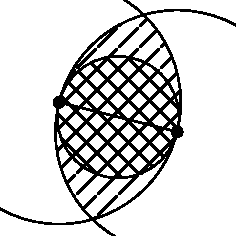
\includegraphics[width=0.14\textwidth]{images/GG_RNG_def}
        }
        \subfigure[]{
            \label{sfig:lunes:rng}
            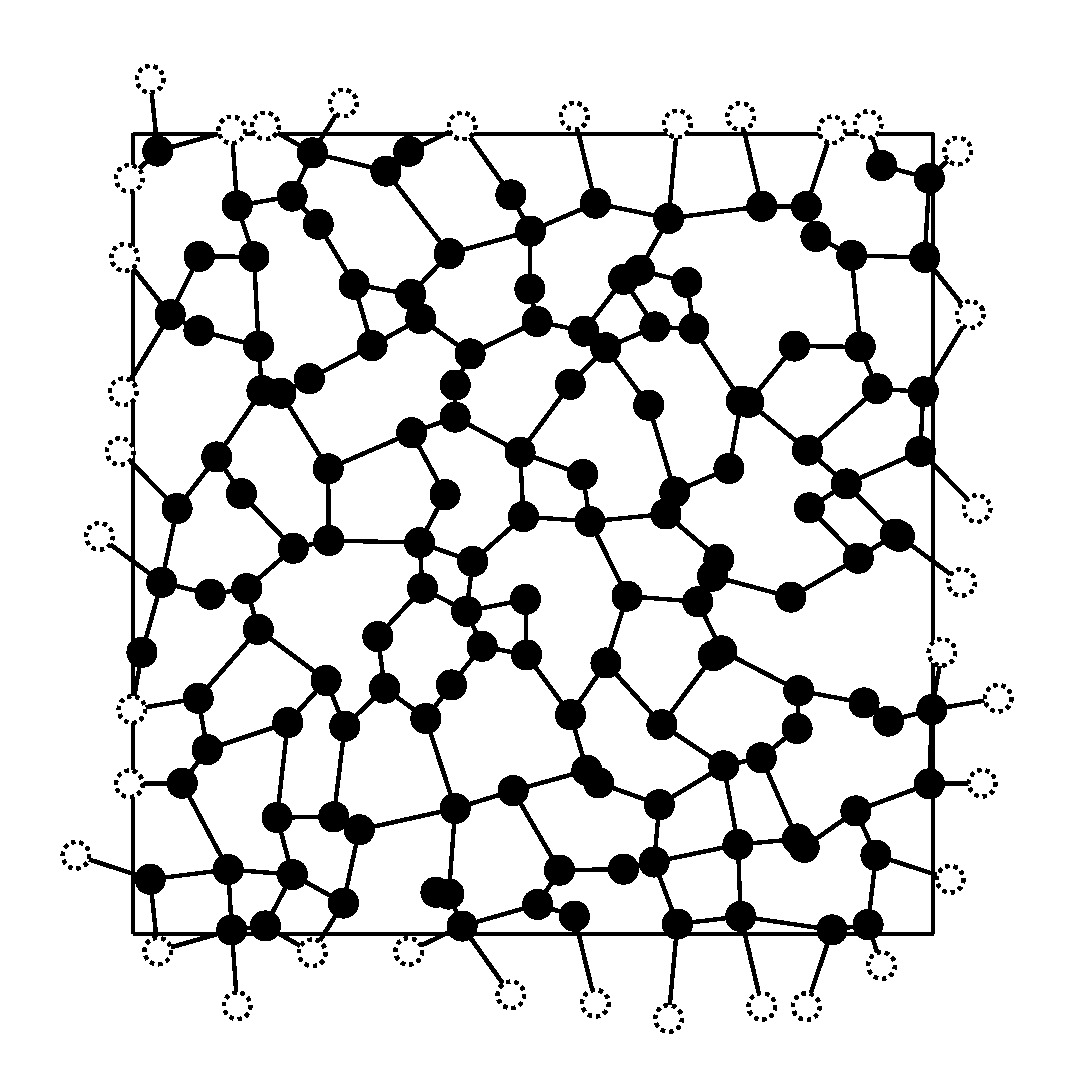
\includegraphics[width=0.14\textwidth]{images/RNG/L12S03}
        }
        \subfigure[]{
            \label{sfig:lunes:gg}
            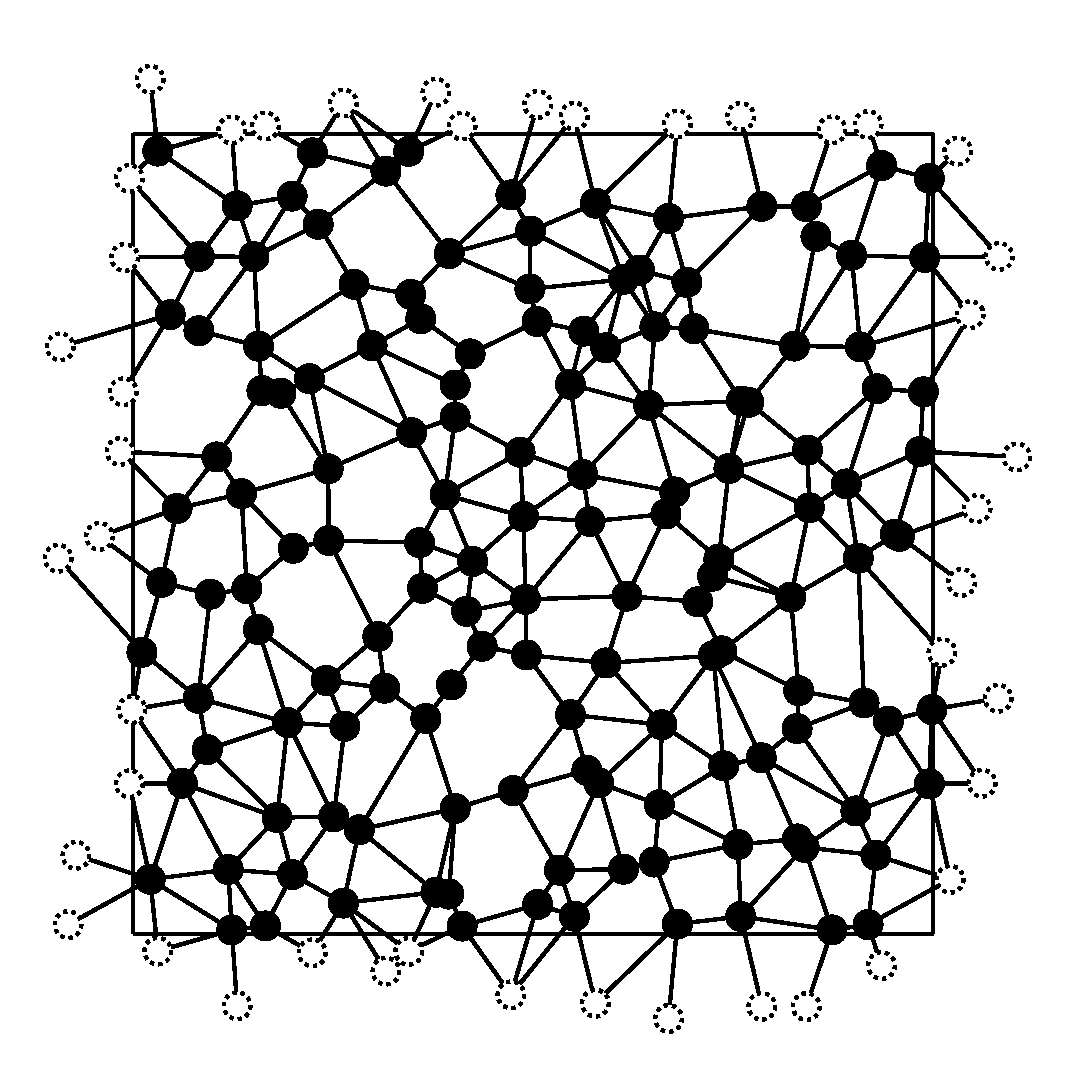
\includegraphics[width=0.14\textwidth]{images/GG/L12S03}
        }
        \caption[Gabriel and Relative Neighborhood Graph]
        {
            \subref{sfig:lunes:def} Lunes, which define whether an edge
                exist, of RNG (hatched region) and GG (cross hatched region).
                It is evident from this sketch that the GG is a supergraph
                of the RNG. If there is an edge in the RNG, the hatched
                region contains no node, then of course also the double
                hatched region contains no node and thus this edge appears
                also in the GG. So every egde of the RNG is also present
                in a GG on the same set of nodes.
            \subref{sfig:lunes:rng} Example of a RNG on periodic
                boundary conditions.
            \subref{sfig:lunes:gg} Example of a GG on
                periodic boundary conditions. Periodic nodes are dashed.
        }
        \label{fig:lunes}
    \end{figure}

    The \emph{Gabriel graph} (GG) \cite{Gabriel1969} is a subgraph
    of the Delaunay triangulation \cite{Delaunay1934,Katajainen}
    (DT), i.e.~for the same set of nodes \(V\) the edge set of the
    DT is a superset of the edge set of the GG. Two nodes \(i\) and
    \(j\) with distance \(d_{ij}\) will be connected with an edge,
    if a circle with its center on half way between \(i\) and \(j\)
    and radius \(r = \frac{d_{ij}}{2}\) contains no other nodes, i.e.~the
    condition
    \[d_{ij} < d_{ik} + d_{kj} \forall k \in V\setminus\{i,j\}\]
    is fulfilled. See
    also the cross hatched region from Fig.~\ref{sfig:lunes:def}. An
    example is given in Fig.~\ref {sfig:lunes:gg}. Note that the
    lune of the GG is completely enclosed in the lune of the RNG,
    therefore the RNG is a subgraph of the GG.

    To construct these graphs there is an algorithm\cite{RNGCell} with
    a time complexity of \(\mathcal{O}(N \log N)\) for nodes on a two
    dimensional plane.

\subsection{The Ising Model}
\label{ssec:model}
    Commonly, the IFM is studies on a square lattice with lateral length
    \(L\) and \(N=L^2\) nodes with periodic boundary conditions.
    Each site $i$ has an Ising spin \(s_i \in \{-1,+1\}\) and interacts with its
    nearest neighbors described by the Hamiltonian
    \begin{equation}
        \mathcal{H} = - \sum_{\avg{i,j}}J_{ij}s_{i}s_{j}.
        \label{eq:hamiltonian}
    \end{equation}
    \(\avg{i,j}\) refers to nodes \(i\) and \(j\) which are
    nearest neighbors, i.e.~they are connected by an edge.
    The coupling strength between \(i\) and \(j\) is given by
    \(J_{ij}\).

    In this article the nodes of the square lattice are
    displaced, introducing geometric disorder resulting in a non regular graph
    structure.
    The displacement is randomly Gaussian distributed with standard
    deviation \(\sigma\), i.e.~the \(x\) and \(y\) coordinates of the
    sites are displaced by random \(\Delta x\) and \(\Delta y\) drawn
    from a Gaussian distribution with zero mean.
    In the following \(\sigma\) will be called \emph{disorder parameter}.
    If we took ``nearest neighbor" in the Euclidean meaning, most sites
    would only have one nearest neighbor after the
    displacement. If only the edges between these neighbors remained,
    the lattice would collapse to many very small clusters. If on the
    other hand all edges remained as they were before the displacement,
    edges might cross each other -- at least for big displacements.
    The crossing of edges would destroy the planar character of the graph.
    To avoid this, a new edge-set will be established after the displacement
    to form a proximity graph. The influence of $\sigma$ on the
    structure of a proximity graph is shown in Fig.~\ref{fig:RNG_sigma}
    for a RNG.
    \begin{figure}[htb]
        \centering
        \subfigure[$\sigma = 0.09$]
        {
            \label{sfig:RNG_sigma:0.09}
            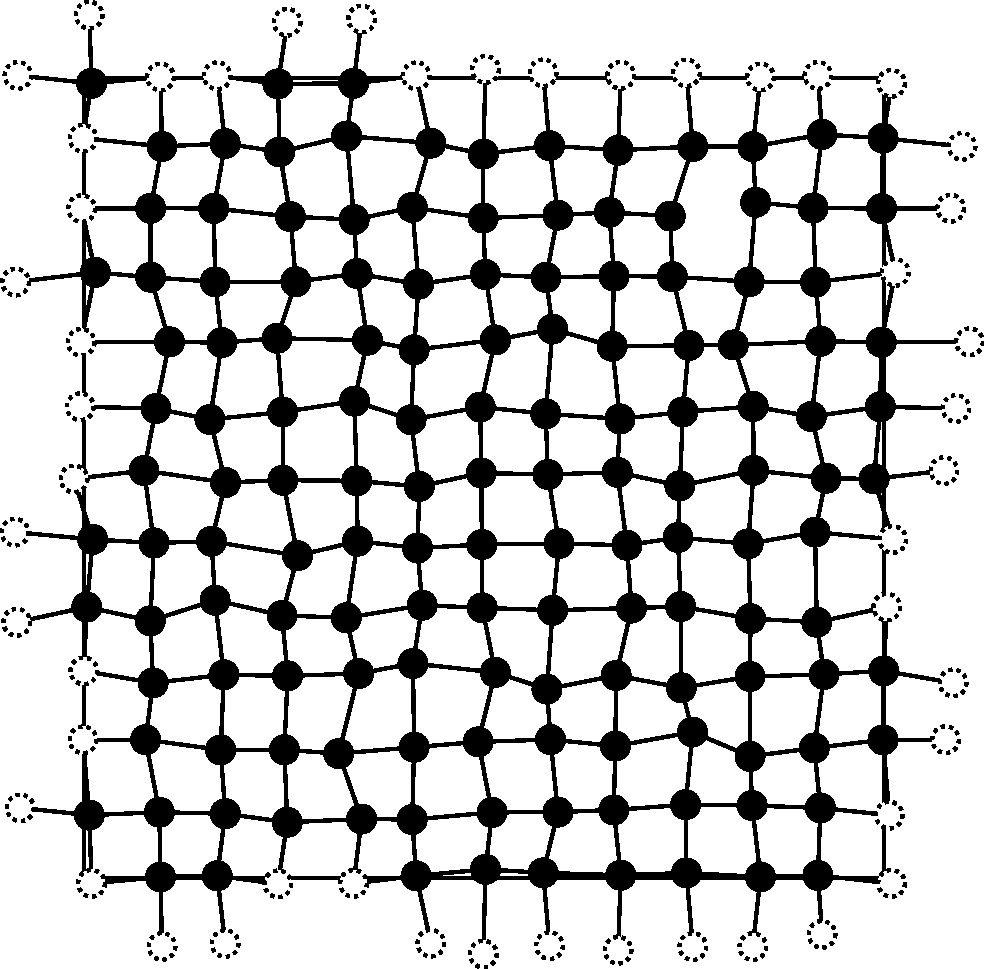
\includegraphics[width=0.14\textwidth]{images/RNG/out009}
        }
        \subfigure[$\sigma = 0.15$]
        {
            \label{sfig:RNG_sigma:0.15}
            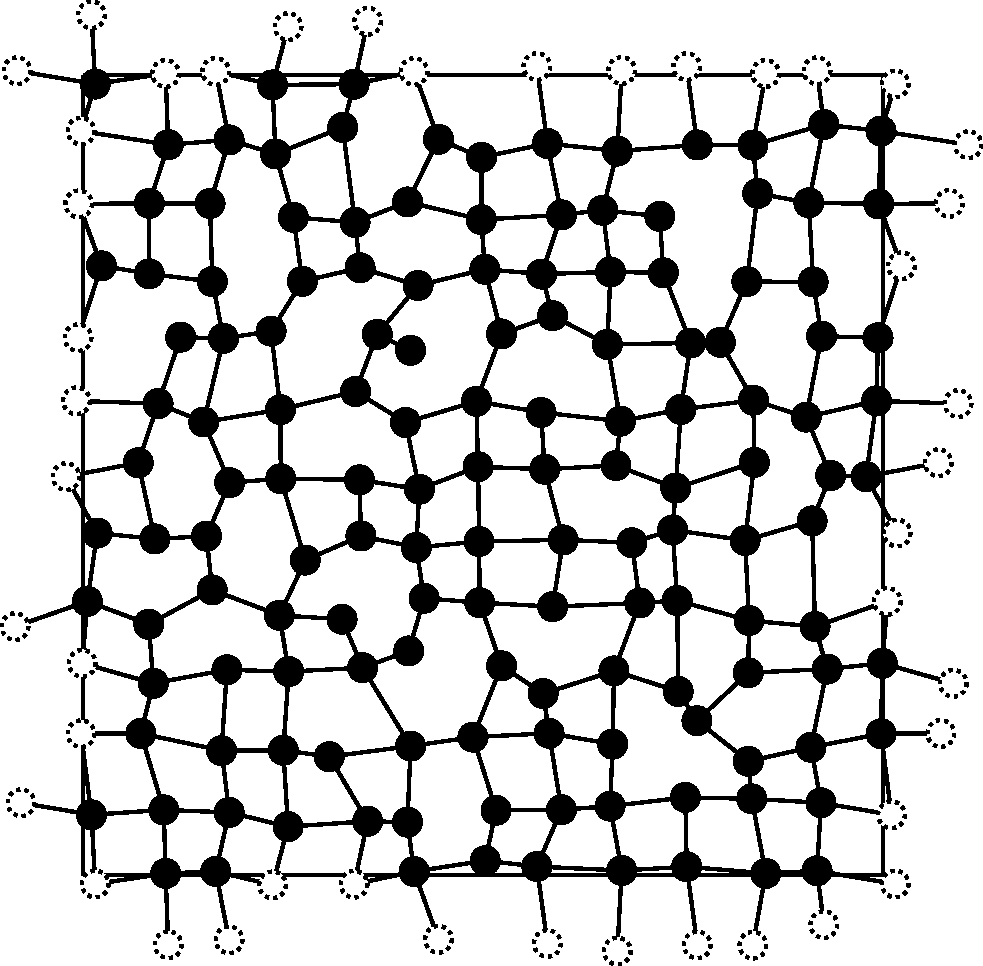
\includegraphics[width=0.14\textwidth]{images/RNG/out015}
        }
        \subfigure[$\sigma = 0.21$]
        {
            \label{sfig:RNG_sigma:0.21}
            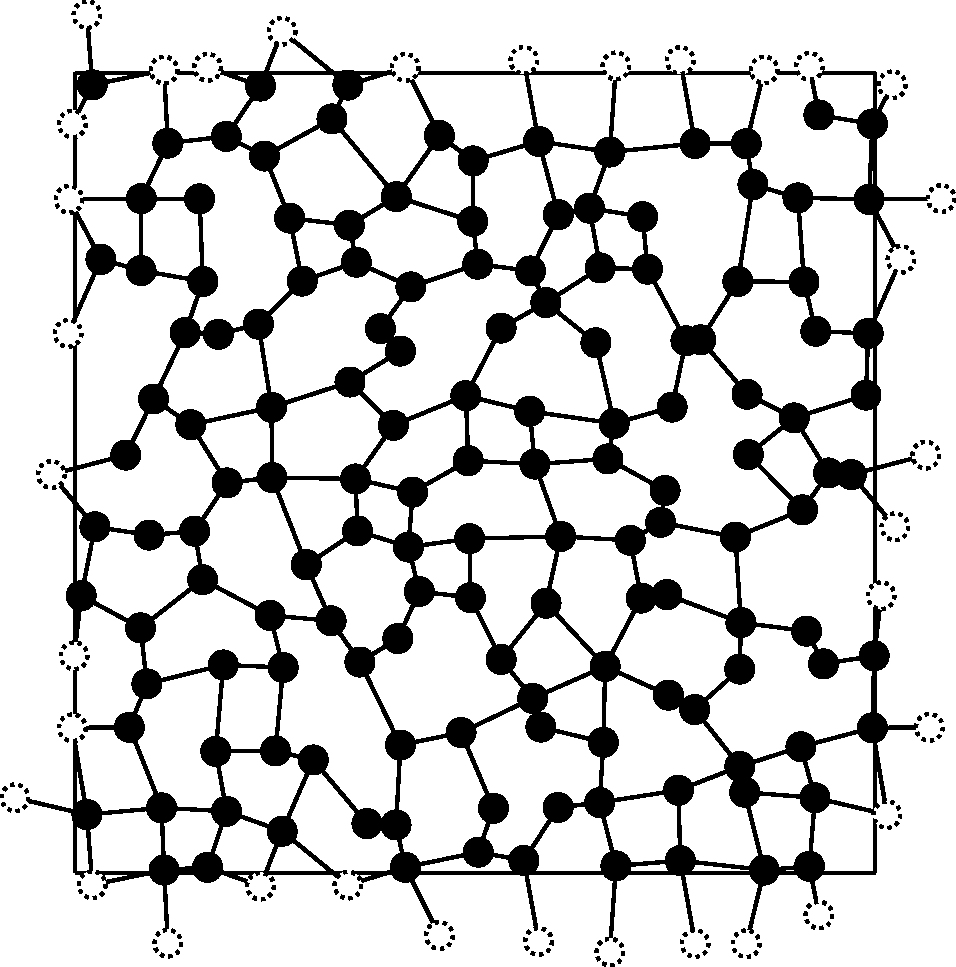
\includegraphics[width=0.14\textwidth]{images/RNG/out021}
        }
        \caption[Examples of RNG for different $\sigma$]
        {
            Examples of proximity graphs (more precise, Relative Neighborhood
            graph see Sec. \ref{ssec:graphtypes}) for different $\sigma$.
            Connections which cross a periodic boundary are indicated
            by edges which connect a solid node to a dashed node.
        }
        \label{fig:RNG_sigma}
    \end{figure}
    The coupling constants \(J_{ij}\), i.e.~edge weights, depend on the
    geometric distance between the connected pair of sites. More precise,
    the weight of an edge is
    \begin{equation}
        E_{ij} = J_{ij} = \mathrm{e}^{\alpha (1-d_{ij})},
        \label{eq:coupling}
    \end{equation}
    where \(d_{ij}\) is the Euclidean
    distance between node \(i\) and \(j\). Following Ref.~\cite{Lima2000}
    the free parameter \(\alpha\) is set to \(\alpha = 0.5\).
    Note that for \(\sigma = 0\) the resulting \(d_{ij} = 1\) and therefore
    \(J_{ij} = 1\) for every edge $\{i,j\}$. Consequently, in this case
    the graph is a common square lattice.
